%% Le lingue utilizzate, che verranno passate come opzioni al pacchetto babel. Come sempre, l'ultima indicata sarà quella primaria.
%% Se si utilizzano una o più lingue diverse da "italian" o "english", leggere le istruzioni in fondo.
\def\thudbabelopt{english,italian}
%% Valori ammessi per target: bach (tesi triennale), mst (tesi magistrale), phd (tesi di dottorato).
%% Valori ammessi per aauheader: '' (vuoto -> nessun header Alpen Adria Univeristat), aics (Department of Artificial Intelligence and Cybersecurity), informatics (Department of Informatics Systems). Il nome del dipartimento è allineato con la versione inglese del logo UniUD.
%% Valori ammessi per style: '' (vuoto -> stile moderno), old (stile tradizionale).
\documentclass[target=bach,aauheader=,style=]{thud}

%% --- Informazioni sulla tesi ---
%% Per tutti i tipi di tesi
% Scommentare quello di interesse, o mettete quello che vi pare
\course{Informatica}
%\course{Internet of Things, Big Data e Web}
%\course{Matematica}
%\course{Comunicazione Multimediale e Tecnologie dell'Informazione}
\title{Un sistema distribuito per l'analisi della topologia di reti di calcolatori}
\author{Diego Cirillo}
\supervisor{Prof.\ Marino Miculan}
\cosupervisor{Dott.\ Matteo Paier}
%\tutor{Guido Necchi}
%% Campi obbligatori: \title, \author e \course.
%% Altri campi disponibili: \reviewer, \tutor, \chair, \date (anno accademico, calcolato in automatico), \rights
%% Con \supervisor, \cosupervisor, \reviewer e \tutor si possono indicare più nomi separati da \and.
%% Per le sole tesi di dottorato:
%\phdnumber{313}
%\cycle{XXVIII}
%\contacts{Via della Sintassi Astratta, 0/1\\65536 Gigatera --- Italia\\+39 0123 456789\\\texttt{http://www.example.com}\\\texttt{inbox@example.com}}

%% --- Pacchetti consigliati ---
%% pdfx: per generare il PDF/A per l'archiviazione. Necessario solo per la versione finale
\usepackage[a-1b]{pdfx}
%% hyperref: Regola le impostazioni della creazione del PDF... più tante altre cose. Ricordarsi di usare l'opzione pdfa.
\usepackage[pdfa]{hyperref}
%% tocbibind: Inserisce nell'indice anche la lista delle figure, la bibliografia, ecc.
\graphicspath{ {./images/} }
%% --- Stili di pagina disponibili (comando \pagestyle) ---
%% sfbig (predefinito): Apertura delle parti e dei capitoli col numero grande; titoli delle parti e dei capitoli e intestazioni di pagina in sans serif.
%% big: Come "sfbig", solo serif.
%% plain: Apertura delle parti e dei capitoli tradizionali di LaTeX; intestazioni di pagina come "big".
\usepackage{placeins}

\begin{document}
\maketitle

%% Dedica (opzionale)
\begin{dedication}
	A questa pagina, \par che mi ha aiutato ad aumentare le pagine totali.
\end{dedication}

% Ringraziamenti (opzionali)
\acknowledgements
Vorrei esprimere un sentito ringraziamento a tutti coloro che mi hanno supportato durante questo percorso. Innanzitutto, un grazie speciale sia al mio relatore che il mio correlatore per la guida e la pazienza. Grazie ai miei compagni di progetto, senza i quali non sarei riuscito a superare le tante sfide incontrate lungo la strada.


Questo progetto ha rappresentato per me una sfida entusiasmante e formativa, poiché è stata la prima volta che ho avuto l'opportunità di lavorare su un'iniziativa di media grandezza insieme ad altre persone. All'inizio, mi sentivo come se fossi in mare aperto, senza una chiara direzione e sopraffatto dalla complessità del lavoro. Il codice da scrivere, le tecnologie da apprendere e la necessità di collaborare efficacemente con il resto del team sembravano compiti immensi e difficili da gestire.


Tuttavia, grazie al sostegno e alla collaborazione degli altri membri del team, sono riuscito a superare queste difficoltà iniziali. Ho avuto l'opportunità di imparare moltissimo, sia dal punto di vista tecnico che umano. Le sfide che mi sembravano insormontabili sono diventate, grazie all'aiuto e alla guida dei miei colleghi, delle opportunità di crescita. La mia conoscenza di Rust è notevolmente migliorata, e ho acquisito una comprensione più profonda delle pratiche di sviluppo collaborativo e delle dinamiche di un progetto su larga scala.


Guardando al percorso che abbiamo compiuto finora, sono estremamente emozionato per come il progetto sta prendendo forma. La nostra architettura sta dimostrando di essere robusta e scalabile, e i miglioramenti che ho contribuito a implementare stanno avendo un impatto tangibile sulla qualità complessiva del sistema.


Ma non è solo il successo tecnico a motivarmi. Lavorare in un team che condivide la mia passione per la tecnologia e l'innovazione è stato incredibilmente gratificante. L'ambiente collaborativo e il continuo scambio di idee hanno reso questo progetto un'esperienza unica e preziosa per il mio sviluppo professionale e personale.


Per il futuro, sono determinato a continuare a contribuire a questo progetto. C'è ancora molto lavoro da fare, molte sfide da affrontare e molte opportunità di miglioramento e innovazione. Sono impaziente di vedere dove ci porterà questo viaggio e sono entusiasta di poter continuare a far parte del team che lo sta rendendo possibile.


In sintesi, questo progetto non è stato solo un'opportunità per applicare e sviluppare le mie competenze tecniche, ma è stato anche un'esperienza di crescita personale. La collaborazione, la condivisione delle conoscenze e il supporto reciproco sono stati elementi chiave per superare le difficoltà iniziali e portare avanti un lavoro di qualità. Sono grato per l'opportunità di far parte di questo team e sono entusiasta di continuare a contribuire al successo del progetto.


Un ringraziamento va anche alla mia famiglia, che mi ha sostenuto in ogni momento, e ai miei amici, per avermi sempre spronato a dare il meglio di me.

%% Sommario (opzionale)
%\abstract
%La crescente complessità delle reti di calcolatori moderne richiede strumenti sofisticati per la loro analisi e gestione. Questa tesi presenta la progettazione e lo sviluppo di un sistema distribuito innovativo, capace di esplorare e mappare in modo efficiente le topologie di reti di grandi dimensioni. Il sistema proposto è in grado di estrarre informazioni significative sulla struttura della rete, identificando pattern, anomalie e potenziali vulnerabilità. L'obiettivo finale è fornire ai network administratori un quadro completo e dettagliato della loro infrastruttura, supportando decisioni informate e ottimizzando le performance della rete.

%% Indice
\tableofcontents

%% Lista delle tabelle (se presenti)
%\listoftables

% Lista delle figure (se presenti)
\listoffigures

%% Corpo principale del documento
\mainmatter

%% Parte
%% La suddivisione in parti è opzionale; solitamente sono sufficienti i capitoli.
%\part{Parte}

%% Capitolo
\chapter{Introduzione}
\section{Motivazioni dello Studio}
\subsection{Importanza dell'analisi della topologia di rete.}
Come descritto in \cite{tanenbaum2011computer} l'analisi della topologia di rete è un'attività cruciale per la gestione, la sicurezza e l'ottimizzazione delle infrastrutture di rete. La topologia di rete rappresenta la struttura fisica e logica di una rete, delineando come i dispositivi (come router, switch, server, ecc.) siano interconnessi e come i dati fluiscano tra di essi. Una comprensione dettagliata della topologia è essenziale per diverse ragioni:
\begin{itemize}
  \item \textbf{Ottimizzazione delle Prestazioni}: Una corretta analisi della topologia consente di identificare colli di bottiglia, percorsi inefficienti e configurazioni subottimali che possono influenzare negativamente le prestazioni della rete. Migliorando la topologia, si possono ottenere connessioni più rapide e una distribuzione del traffico più bilanciata.
  \item \textbf{Gestione e Manutenzione}: Conoscere la topologia della rete permette agli amministratori di pianificare meglio le operazioni di manutenzione, minimizzando i tempi di inattività e assicurando la continuità dei servizi. Inoltre, facilita la gestione delle risorse di rete, come l'allocazione degli indirizzi IP e la configurazione dei dispositivi.
  \item \textbf{Sicurezza}: L'analisi della topologia di rete è fondamentale per la sicurezza. Permette di identificare punti deboli nella struttura della rete, come collegamenti non protetti o dispositivi non autorizzati. Questo consente di implementare misure di sicurezza più efficaci, come firewall e segmentazioni di rete.
  \item \textbf{Rilevamento e Risoluzione dei Problemi}: In caso di problemi di rete, una mappa precisa della topologia aiuta a individuare rapidamente la causa dei malfunzionamenti, facilitando una risoluzione tempestiva e riducendo i tempi di inattività.
  \item \textbf{Scalabilità}: Una buona comprensione della topologia è essenziale quando si vuole espandere la rete. Aiuta a garantire che l'espansione avvenga in modo efficiente, senza compromettere le prestazioni o la sicurezza della rete.
\end{itemize}

\subsection{Scopi e obiettivi della tesi.}
La tesi ha come scopo principale la progettazione e lo sviluppo di un sistema distribuito innovativo per l'analisi della topologia di reti di calcolatori, che superi i limiti degli strumenti attualmente disponibili, come SNMP (Simple Network Management Protocol) e altri metodi tradizionali.
\newline
Obiettivi Specifici:
\begin{itemize}
  \item \textbf{Identificazione delle Limitazioni degli Strumenti Esistenti}:
    \begin{itemize}
      \item Analizzare i principali strumenti attualmente utilizzati per l'analisi della topologia di rete, evidenziando le loro carenze in termini di accuratezza, scalabilità, efficienza e sicurezza.
    \item Evidenziare in particolare i limiti di SNMP, come la sua dipendenza da dati statici, la mancanza di supporto per reti complesse e l'inefficienza nella gestione di grandi volumi di dati in tempo reale.
    \end{itemize}

  \item \textbf{Progettazione di un'Architettura Distribuita}:
    \begin{itemize}
      \item Sviluppare un'architettura di sistema distribuita che permetta un'analisi più accurata e dinamica della topologia di rete.
      \item Garantire che il sistema sia scalabile e in grado di gestire grandi reti eterogenee, mantenendo un basso impatto sulle risorse di rete.
    \end{itemize}
    
  %\item Sviluppo di Algoritmi Innovativi:
  %  \begin{itemize}
  %    \item Progettare e implementare algoritmi avanzati per il rilevamento e l'analisi della topologia, che siano in grado di adattarsi dinamicamente ai cambiamenti della rete.
  %    \item Migliorare l'efficienza del sistema, riducendo la latenza e ottimizzando l'uso delle risorse.
  %  \end{itemize}

  %\item Valutazione delle Prestazioni:
  %  \begin{itemize}
  %    \item Confrontare le prestazioni del sistema proposto con quelle degli strumenti esistenti, utilizzando criteri come accuratezza della mappatura, tempo di risposta, utilizzo delle risorse e sicurezza.
  %    \item Testare il sistema in diversi scenari reali per valutarne l'efficacia e identificare eventuali aree di miglioramento.
  %  \end{itemize}


  \item \textbf{Contributo alla Comunità Scientifica e Industriale}:
    \begin{itemize}
      \item Fornire una soluzione innovativa che possa essere utilizzata in ambito accademico e industriale per migliorare la gestione e la sicurezza delle reti di calcolatori.
      \item Contribuire alla letteratura esistente con nuove metodologie e strumenti per l'analisi della topologia di rete.
    \end{itemize}

\end{itemize}



\section{Struttura della Tesi}
Questa tesi è organizzata in 7 capitoli, ciascuno dei quali affronta aspetti fondamentali dello sviluppo e dell'analisi di un sistema distribuito per l'analisi della topologia di reti di calcolatori. Di seguito viene presentata una panoramica della struttura della tesi.

\begin{itemize}
  \item \textbf{Capitolo 1: Introduzione}
  \begin{itemize}
    \item[] Questo capitolo introduce il tema centrale della tesi, evidenziando l'importanza dell'analisi della topologia di rete. Vengono inoltre delineati gli scopi e gli obiettivi del lavoro, insieme alla struttura generale della tesi.
  \end{itemize}


\item \textbf{Capitolo 2: Breve panoramica sui metodi di analisi di rete}
    \begin{itemize}
      \item[] Nel secondo capitolo vengono esaminati i concetti fondamentali di topologia di rete e vengono descritti i metodi comuni utilizzati per la sua analisi. Viene inoltre condotta un'analisi critica degli strumenti attualmente disponibili, con particolare attenzione ai loro limiti e alle carenze, soprattutto riguardo a SNMP.
    \end{itemize}


  \item \textbf{Capitolo 3: Requisiti di un sistema distribuito di mappatura di reti informatiche}
    \begin{itemize}
      \item[] In questo capitolo vengono discussi in dettaglio i problemi principali che emergono dall'utilizzo degli strumenti esistenti per l'analisi della topologia di rete. Vengono quindi identificati e descritti i requisiti in termini di accuratezza, scalabilità, latenza, efficienza, sicurezza e privacy che un buon sistema per l'analisi di rete dovrebbe avere.
    \end{itemize}


  \item \textbf{Capitolo 4: Progettazione del Sistema}
    \begin{itemize}
      \item[] Il quarto capitolo descrive la soluzione proposta e in dettaglio l'architettura del sistema, i protocolli di comunicazione utilizzati, gli algoritmi sviluppati per l'analisi della topologia e le misure di sicurezza adottate. Viene fornita una descrizione tecnica della progettazione del sistema, enfatizzando le soluzioni innovative implementate.
    \end{itemize}


  \item \textbf{Capitolo 5: Il modulo Executer}
    \begin{itemize}
      \item[] Questo capitolo descrive l'architettura dell'Executer, il componente centrale responsabile della gestione e coordinazione delle operazioni di scansione sulla rete, e analizza in dettaglio come comunica con gli altri moduli tramite un sistema di messaggistica basato su canali FIFO e MQTT.
    \end{itemize}


  \item \textbf{Capitolo 6: Implementazione del modulo Executer}
    \begin{itemize}
      \item[] In questo capitolo vengono presentate le scelte tecniche e di implementazione dell'Executer, comprese le librerie utilizzate in Rust, la gestione della comunicazione tra moduli tramite MQTT e l'infrastruttura basata su Mosquitto per coordinare le scansioni e raccogliere i risultati.
    \end{itemize}

  \item \textbf{Capitolo 7: Conclusioni}
    \begin{itemize}
      \item[] L'ultimo capitolo riflette sul mio percorso personale durante lo sviluppo del progetto sottolineando l'importanza della collaborazione e del lavoro di squadra nel raggiungimento dei risultati ottenuti. 
    \end{itemize}

\end{itemize}


%\chapter{Stato dell'Arte}
\chapter{Breve panoramica sui metodi di analisi di rete}
\label{art}
\section{Metodi comuni di analisi della topologia.}
L'analisi della topologia di rete implica l'identificazione, la mappatura e la valutazione della struttura della rete, al fine di ottimizzarne il funzionamento e la gestione. Ecco i metodi più comuni utilizzati per questa analisi:
\subsubsection{SNMP (Simple Network Management Protocol)} 
SNMP (Simple Network Management Protocol) \cite{rfc1157} è un protocollo standardizzato progettato per la gestione e il monitoraggio dei dispositivi di rete. Funziona attraverso una struttura di gestione che include agenti e manager: gli agenti sono software installati sui dispositivi di rete, come router e switch, e si occupano di raccogliere e memorizzare informazioni riguardanti lo stato e le prestazioni di tali dispositivi. I manager, d'altra parte, sono applicazioni che interrogano gli agenti per ottenere i dati necessari. Questi dati sono organizzati in una MIB (Management Information Base) \cite{rfc1213}, una struttura che rappresenta ogni oggetto di rete con un identificatore unico.

Il protocollo è relativamente semplice da configurare e gestire, anche per amministratori di rete meno esperti. Inoltre, SNMP è ampiamente supportato da una vasta gamma di dispositivi di rete, facilitando l'integrazione in ambienti di rete diversi. Il protocollo consente un monitoraggio e una gestione dettagliati di vari aspetti della rete, inclusi le prestazioni e lo stato dei dispositivi, contribuendo a mantenere l'efficienza e la disponibilità della rete.

La sua capacità di rilevare dinamicamente i cambiamenti nella topologia della rete è limitata, il che può ridurre l'efficacia del protocollo in ambienti molto dinamici. Inoltre, in reti complesse o eterogenee, l'analisi dei dati raccolti può diventare complicata, richiedendo strumenti avanzati per una corretta interpretazione. Infine, con l'aumentare delle dimensioni della rete, la scalabilità di SNMP può rappresentare un problema, poiché la gestione di un numero molto elevato di dispositivi può mettere a dura prova le capacità del manager e rendere più complessa la configurazione degli agenti.

\subsubsection{Traceroute}
Traceroute \cite{netbrain_traceroute} è uno strumento diagnostico fondamentale utilizzato per analizzare il percorso dei pacchetti di dati attraverso una rete IP fino a una destinazione specifica. Funziona inviando pacchetti con tempi di vita (TTL) crescenti e misurando il tempo impiegato per ottenere una risposta da ciascun router intermedio. Questo processo consente di identificare tutti i router attraversati dal pacchetto, fornendo così una visione dettagliata del percorso seguito dai dati.

Permette di individuare i punti di congestione o i router che potrebbero essere malfunzionanti, facilitando così l’individuazione di problemi specifici lungo il percorso dei dati. Inoltre, offre una panoramica utile dei percorsi che i dati percorrono tra i diversi dispositivi, contribuendo a una migliore comprensione della rete e delle sue dinamiche.

È specificamente progettato per le reti IP, il che significa che non può essere utilizzato per diagnosticare problemi su reti non IP o su reti miste. Inoltre, non fornisce una visione completa della topologia della rete; si limita a mostrare il percorso dei pacchetti tra due punti senza considerare altri aspetti della rete, come la sua struttura complessiva. Infine, Traceroute può essere bloccato o filtrato da firewall e altri dispositivi di sicurezza, il che può impedire la raccolta di dati accurati e limitare l’efficacia dello strumento in ambienti protetti.

\subsubsection{NetFlow/IPFIX}
NetFlow \cite{cisco_netflow}, insieme alla sua evoluzione IPFIX (Internet Protocol Flow Information Export) \cite{rfc7011}, è un protocollo sviluppato da Cisco per raccogliere e analizzare informazioni sui flussi di dati che transitano attraverso un router o uno switch di rete. Questo protocollo si concentra sull'acquisizione di dettagli relativi alle conversazioni tra dispositivi di rete, come indirizzi IP sorgente e destinazione, porte utilizzate, e volume di dati scambiati. NetFlow e IPFIX sono strumenti essenziali per il monitoraggio e la gestione delle reti, poiché forniscono una visione approfondita delle comunicazioni di rete e del traffico.

Questi protocolli consentono di effettuare analisi approfondite del traffico, identificare pattern di utilizzo, e rilevare anomalie che potrebbero indicare problemi come congestionamenti, attacchi DDoS o comportamenti non autorizzati. Le informazioni fornite da NetFlow e IPFIX possono essere utilizzate per ottimizzare le prestazioni della rete, migliorare la sicurezza e pianificare l'espansione della rete in modo informato.

Non forniscono direttamente una mappa della topologia di rete; piuttosto, si concentrano sui flussi di traffico, il che significa che non mostrano come i dispositivi sono connessi tra loro. Inoltre, la raccolta e l'analisi dei dati tramite questi protocolli richiedono significative risorse di elaborazione e archiviazione. La quantità di dati generata può essere molto elevata, specialmente in reti con elevato traffico, e richiede quindi sistemi di gestione e storage capaci di gestire grandi volumi di informazioni.

\subsubsection{LLDP (Link Layer Discovery Protocol)}
LLDP (Link Layer Discovery Protocol) \cite{ieee_lldp} è un protocollo di livello datalink progettato per facilitare la scoperta dei dispositivi di rete vicini e per la condivisione di informazioni riguardanti la loro configurazione. Operando al livello 2 del modello OSI, LLDP permette ai dispositivi di rete, come switch e router, di annunciare e scoprire informazioni sui dispositivi a loro collegati attraverso l'invio di pacchetti di dati. Questi pacchetti contengono dettagli utili, come l'identificativo del dispositivo, le sue capacità e il suo stato di configurazione, consentendo una visione più chiara dei dispositivi connessi direttamente alla stessa rete.

Uno dei principali vantaggi di LLDP è la sua capacità di automatizzare la scoperta dei dispositivi di rete. Questo processo semplifica la gestione della rete, poiché consente agli amministratori di ottenere informazioni aggiornate e precise sui dispositivi senza la necessità di una configurazione manuale dettagliata. Inoltre, la possibilità di condividere informazioni di configurazione aiuta nella gestione e nella risoluzione dei problemi della rete, migliorando la visibilità e la comprensione delle connessioni fisiche e delle relazioni tra i dispositivi.

Operando esclusivamente al livello 2 del modello OSI, il protocollo è confinato al livello di collegamento dati e non offre una visione completa della topologia a livello IP o superiore. Ciò significa che, mentre LLDP è efficace nel fornire dettagli sui dispositivi locali e le loro connessioni, non può fornire informazioni sulla topologia della rete a livello di rete (IP) o di livello superiore. Di conseguenza, per ottenere una panoramica completa della rete e delle sue connessioni a livello più alto, potrebbero essere necessari ulteriori strumenti e protocolli.
\newline
\newline
Questi metodi offrono diverse prospettive sull'analisi della topologia di rete, ognuno con i propri punti di forza e debolezze. Tuttavia, nessuno di essi, preso singolarmente, offre una soluzione completa per l'analisi della topologia di reti complesse e dinamiche, evidenziando la necessità di strumenti più avanzati e integrati.

\section{Problemi dell'utilizzo di SNMP per l'Analisi della Topologia}
SNMP (Simple Network Management Protocol) è uno dei protocolli più utilizzati per il monitoraggio e la gestione delle reti, ma presenta diversi limiti significativi quando viene utilizzato per l'analisi della topologia di rete. Di seguito vengono analizzati i principali problemi associati all'uso di SNMP in questo contesto.

\subsubsection{Scalabilità Limitata}
    \begin{itemize}
      \item \textbf{Overhead di Polling}: SNMP si basa su un meccanismo di polling, in cui un sistema di gestione della rete (NMS) invia richieste ai dispositivi per ottenere informazioni sul loro stato. In una rete di grandi dimensioni, il numero di richieste necessarie per raccogliere i dati da tutti i dispositivi può diventare ingente, causando un significativo overhead di rete e aumentando il carico sui dispositivi stessi.
      \item \textbf{Crescita Esponenziale del Traffico di Gestione}: Man mano che il numero di dispositivi in rete aumenta, anche il volume del traffico di gestione generato da SNMP cresce esponenzialmente, rischiando di congestionare la rete e rallentare le operazioni di monitoraggio.
    \end{itemize}

\subsubsection{ Visione Statica della Topologia}
  \begin{itemize}
    \item \textbf{Informazioni Non in Tempo Reale}: Poiché SNMP si basa su un ciclo di polling, i dati raccolti rappresentano istantanee dello stato della rete in momenti specifici. Questo significa che i cambiamenti dinamici nella topologia, come l'aggiunta o la rimozione di dispositivi, potrebbero non essere rilevati immediatamente, portando a una rappresentazione obsoleta della rete.
    \item \textbf{Mancanza di Rilevamento dei Cambiamenti Dinamici}: In reti moderne, dove la topologia può cambiare rapidamente a causa della virtualizzazione, del cloud computing o delle configurazioni dinamiche, SNMP non riesce a rilevare e adattarsi efficacemente a questi cambiamenti.
  \end{itemize}


\subsubsection{Sicurezza Limitata}
    \begin{itemize}
      \item \textbf{Vulnerabilità di SNMPv1 e SNMPv2}: Le prime versioni di SNMP (v1 e v2) non supportano meccanismi di sicurezza robusti, come l'autenticazione o la crittografia. Le informazioni vengono trasmesse in chiaro, rendendo la rete vulnerabile a intercettazioni e attacchi man-in-the-middle.
      \item \textbf{Complessità di SNMPv3}: Sebbene SNMPv3 introduca miglioramenti significativi in termini di sicurezza, includendo l'autenticazione e la crittografia, la sua implementazione è complessa e richiede una configurazione accurata per essere efficace. La complessità può scoraggiare la piena adozione o portare a configurazioni non sicure.
    \end{itemize}

\subsubsection{Complessità di Configurazione e Manutenzione}
    \begin{itemize}
      \item \textbf{Configurazione Manuale}: Per ottenere una visione accurata della topologia, ogni dispositivo deve essere configurato per rispondere alle richieste SNMP, e questa configurazione deve essere mantenuta e aggiornata nel tempo. In grandi reti, questo può diventare un compito oneroso.
      \item \textbf{Varianza di Supporto tra Vendor}: Non tutti i dispositivi di rete supportano SNMP nello stesso modo, e le implementazioni possono variare tra i diversi vendor, portando a problemi di interoperabilità e difficoltà nel mantenere una mappa coerente della rete.
    \end{itemize}

\subsubsection{Limitata Capacità di Mappatura della Topologia}
    \begin{itemize}
      \item \textbf{Dati Limitati sulla Connettività}: SNMP è utile per raccogliere dati su singoli dispositivi, come lo stato delle interfacce, l'uso della CPU o della memoria, ma non fornisce informazioni dettagliate sulle connessioni tra i dispositivi. Questo rende difficile ottenere una mappa completa e accurata della topologia della rete.
      \item \textbf{Assenza di Informazioni di Layer 2}: SNMP è principalmente focalizzato sui dati di Layer 3 (IP), mancando spesso le informazioni di Layer 2 (Ethernet), che sono cruciali per una mappatura dettagliata della topologia di rete, specialmente in ambienti complessi con VLAN e altri segmenti logici.
    \end{itemize}


\subsubsection{Problemi di Performance}
    \begin{itemize}
      \item \textbf{Impatto sulle Risorse del Dispositivo}: L'elaborazione delle richieste SNMP può consumare risorse significative del dispositivo, specialmente su dispositivi con capacità hardware limitate. Questo può degradare le prestazioni del dispositivo stesso, influenzando la qualità del servizio di rete.
      \item \textbf{Ritardi nella Raccolta dei Dati}: In reti con molti dispositivi o con un utilizzo intensivo di SNMP, i ritardi nella raccolta e nell'analisi dei dati possono aumentare, rendendo meno tempestive le informazioni disponibili e, di conseguenza, meno utile l'analisi della topologia.
    \end{itemize}

\chapter{Requisiti di un sistema distribuito di mappatura di reti informatiche}
Per garantire una mappatura accurata ed efficiente della topologia di rete, un buon sistema di analisi dovrebbe soddisfare una serie di requisiti fondamentali. Questi requisiti derivano dagli svantaggi riscontrati negli strumenti esistenti, come SNMP.

\begin{description}
  \item[Scalabilità]
  Il sistema deve essere in grado di gestire reti di dimensioni variabili, dalla piccola rete locale fino a infrastrutture complesse e distribuite su scala geografica. È essenziale che il sistema possa espandersi senza perdere efficienza e senza introdurre colli di bottiglia man mano che il numero di dispositivi e sottoreti cresce.

  \item[Distribuzione del carico]
  Un buon sistema dovrebbe essere in grado di distribuire il carico di lavoro tra più nodi o moduli, per garantire che l'analisi non sia concentrata su un unico punto. Questo aiuta a evitare situazioni di sovraccarico e assicura che le risorse di rete vengano utilizzate in modo ottimale.

  \item[Bassa latenza e alta efficienza]
  Il sistema deve poter rispondere rapidamente alle richieste e aggiornare la topologia della rete in tempo quasi reale. In una rete dinamica, dove i dispositivi possono connettersi o disconnettersi frequentemente, la capacità di reagire in modo tempestivo è cruciale. Allo stesso tempo, il sistema deve minimizzare l'impatto delle sue operazioni sulla rete monitorata, evitando di introdurre latenza o carico eccessivo.

  \item[Accuratezza]
  La rappresentazione della topologia deve essere il più possibile fedele alla realtà. Ciò significa che il sistema deve essere in grado di rilevare non solo la presenza dei dispositivi, ma anche le loro connessioni, ruoli e attributi, con un livello di dettaglio elevato. Un aspetto cruciale è che il sistema riesca a scoprire e interpretare correttamente i dispositivi eterogenei, indipendentemente dalla loro posizione nella rete.

  \item[Affidabilità e tolleranza ai guasti]
  Dato che un sistema distribuito potrebbe essere soggetto a guasti di rete o problemi locali nei dispositivi di analisi, è essenziale che il sistema sia resiliente. Deve continuare a funzionare, anche in presenza di malfunzionamenti parziali, senza compromettere l'accuratezza o la continuità delle operazioni.

  \item[Modularità e facilità di aggiornamento]
  Un buon sistema deve essere progettato in modo modulare, consentendo di aggiungere o rimuovere facilmente componenti senza impattare sull'intero sistema. Questo approccio facilita gli aggiornamenti, permettendo di introdurre nuovi algoritmi o metodi di analisi man mano che la rete evolve o emergono nuove esigenze.

  \item[Efficienza della comunicazione]
  La comunicazione tra i vari componenti del sistema deve essere efficiente e basata su protocolli standard. In un sistema distribuito, è importante ridurre al minimo la latenza nella trasmissione dei dati tra i diversi moduli di analisi, garantendo che le informazioni vengano propagate e aggregate senza ritardi eccessivi.

\item[Flessibilità di vari protocolli e Strumenti]
    Il sistema dovrebbe essere in grado di adattarsi all'uso di diversi strumenti di analisi e scansione. Questo garantisce una maggiore copertura delle situazioni e permette di sfruttare le potenzialità di strumenti differenti a seconda delle esigenze specifiche della rete monitorata

  \item[Riduzione delle limitazioni dei protocolli tradizionali]
  Molti strumenti tradizionali, come SNMP, soffrono di limitazioni in termini di accuratezza e copertura della rete, non riuscendo a rappresentare correttamente la topologia o a gestire scenari di rete più complessi. Un buon sistema dovrebbe superare questi limiti, fornendo una visione dettagliata e comprensiva della rete senza dipendere da protocolli legacy con capacità limitate

  \item[Sicurezza nelle comunicazioni]
  Le operazioni di analisi della topologia devono avvenire in un ambiente sicuro, proteggendo i dati scambiati tra i vari moduli del sistema. È essenziale garantire l'integrità e la riservatezza delle informazioni raccolte e trasmesse durante il monitoraggio della rete, in particolare in contesti dove si monitorano reti sensibili o ad alto valore strategico.

\end{description}

\section{Conclusioni}

In sintesi, un sistema per l'analisi della topologia di rete deve essere progettato per operare in modo efficiente, scalabile e affidabile, con un forte focus sulla distribuzione del carico, l'accuratezza dei dati raccolti e la resilienza del sistema nel suo complesso. Rispondendo a questi requisiti, si possono ottenere risultati migliori rispetto agli strumenti tradizionali, soprattutto in reti complesse o in continua evoluzione.

\chapter{Progettazione del Sistema}

\section{Soluzione proposta}
Il sistema proposto per l'analisi della topologia di rete è basato su un'architettura distribuita che sfrutta un insieme di probes (sonde) per scansionare contemporaneamente diverse sezioni della rete. Ogni probe utilizza Nmap per raccogliere informazioni dettagliate, che vengono poi aggregate in un database centralizzato. Questo approccio consente di ottenere una visione completa e accurata della topologia di rete, superando i limiti di scalabilità e accuratezza degli strumenti tradizionali.

Nell'architettura proposta, i probes sono distribuiti strategicamente all'interno della rete, con ciascuno di essi responsabile di una specifica area. Operando simultaneamente, i probes eseguono scansioni parallele, raccogliendo dati sui dispositivi di rete, sulle connessioni e sui servizi attivi. I dati raccolti vengono inviati a un database centralizzato, dove vengono normalizzati e aggregati per creare una mappa coerente e dettagliata della rete. L'architettura include anche un sistema di visualizzazione interattivo che permette agli amministratori di esplorare la topologia in tempo reale, monitorando le modifiche e aggiornando continuamente le informazioni.

Uno dei principali vantaggi di questo sistema è la sua scalabilità. A differenza degli approcci centralizzati, che possono soffrire di colli di bottiglia man mano che la rete cresce, l'uso di probes distribuiti consente di gestire efficacemente anche le reti più estese. L'elaborazione parallela delle scansioni riduce il tempo necessario per mappare l'intera rete, distribuendo il carico di lavoro e prevenendo sovraccarichi sui singoli dispositivi.

Un altro vantaggio significativo riguarda l'accuratezza dei dati raccolti. Poiché ogni probe ha una visione dettagliata della porzione di rete che gli è assegnato, il sistema garantisce una copertura completa e precisa della topologia. Inoltre, il processo di aggregazione centralizzato consente di risolvere eventuali discrepanze nei dati e di eliminare le ridondanze, fornendo una rappresentazione accurata e aggiornata della rete.

L'architettura proposta offre anche maggiore resilienza rispetto ai sistemi tradizionali. Se uno o più probes dovessero fallire, il sistema può continuare a funzionare con i probes rimanenti, garantendo la continuità operativa. Inoltre, il sistema è altamente flessibile: può essere facilmente adattato per includere nuovi probes o per modificare l'area di scansione di quelle esistenti, rendendolo capace di rispondere rapidamente ai cambiamenti nella rete.

Dal punto di vista della sicurezza, il sistema è progettato per ridurre al minimo l'esposizione a potenziali attacchi. I dati raccolti vengono trasmessi al database centrale utilizzando canali sicuri e crittografati, proteggendo le informazioni sensibili da eventuali intercettazioni.

In sintesi, l'architettura distribuita proposta rappresenta un significativo miglioramento rispetto agli strumenti tradizionali di analisi della topologia di rete. Essa combina scalabilità, accuratezza, resilienza e sicurezza, offrendo una soluzione completa per la mappatura e il monitoraggio delle reti moderne.

\newpage
\section{Architettura del Sistema}
\subsection{Descrizione dettagliata dell'architettura distribuita}
Il sistema è composto da una architettura client-server \cite{orfali1999client} nella quale il backend si occupa di fare le scansioni, di salvarne i risultati e di fornirli al frontend dove possono essere visualizzati dagli utenti dovrebbero interagire solo con esso. 
Il sistema è basato su un'architettura client-server, un modello classico in cui due entità principali, il client e il server, interagiscono per eseguire e fornire servizi. In questo contesto, il backend agisce come il server, occupandosi delle scansioni di rete e dell'archiviazione dei risultati in un database. Il frontend, che rappresenta il client, richiede i dati al backend per visualizzare i risultati e interagire con essi, fornendo all'utente finale l'interfaccia per analizzare la topologia di rete e i dati raccolti.
L'architettura client-server è un modello distribuito in cui il server fornisce risorse o servizi e il client li utilizza. Il client è tipicamente un'applicazione che invia richieste al server per ottenere informazioni o eseguire azioni. Il server, a sua volta, elabora le richieste, esegue i compiti necessari (come scansioni o elaborazioni dei dati), e risponde al client fornendo i risultati o i dati richiesti.


\begin{figure}[t]
  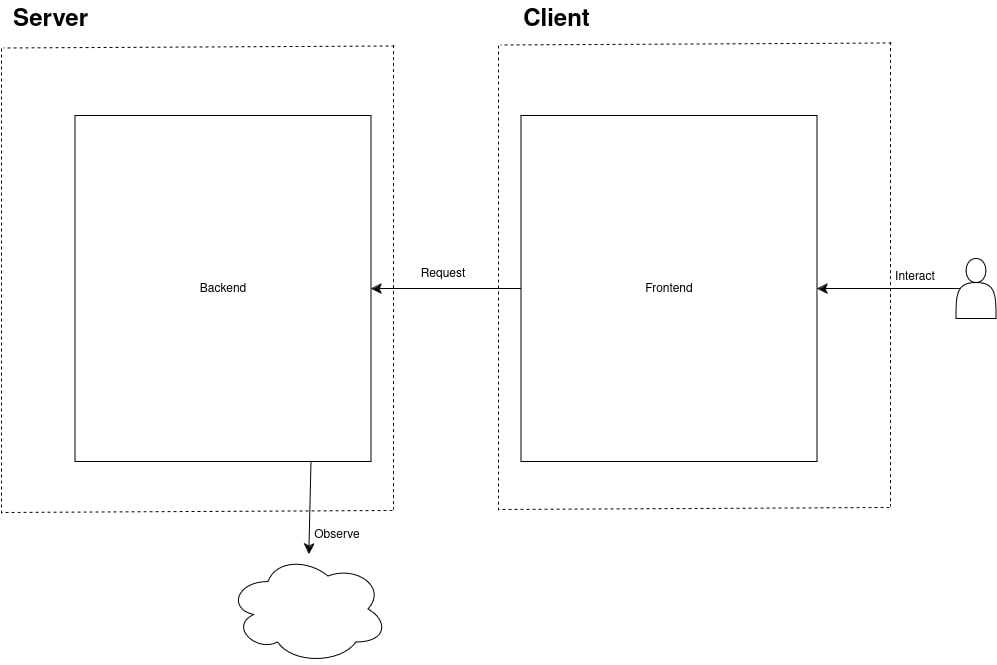
\includegraphics[width=\columnwidth]{client_server}
  \centering
  \caption{Client-Server}
  \label{client-server}
\end{figure}

\FloatBarrier

Come osservabile dalla Figura 4.2 il sistema è diviso in 6 moduli principali su cui ogni componente ha un ruolo specifico per garantire il corretto funzionamento del processo di scansione, elaborazione e analisi dei dati di rete. 


\begin{figure}[t]
  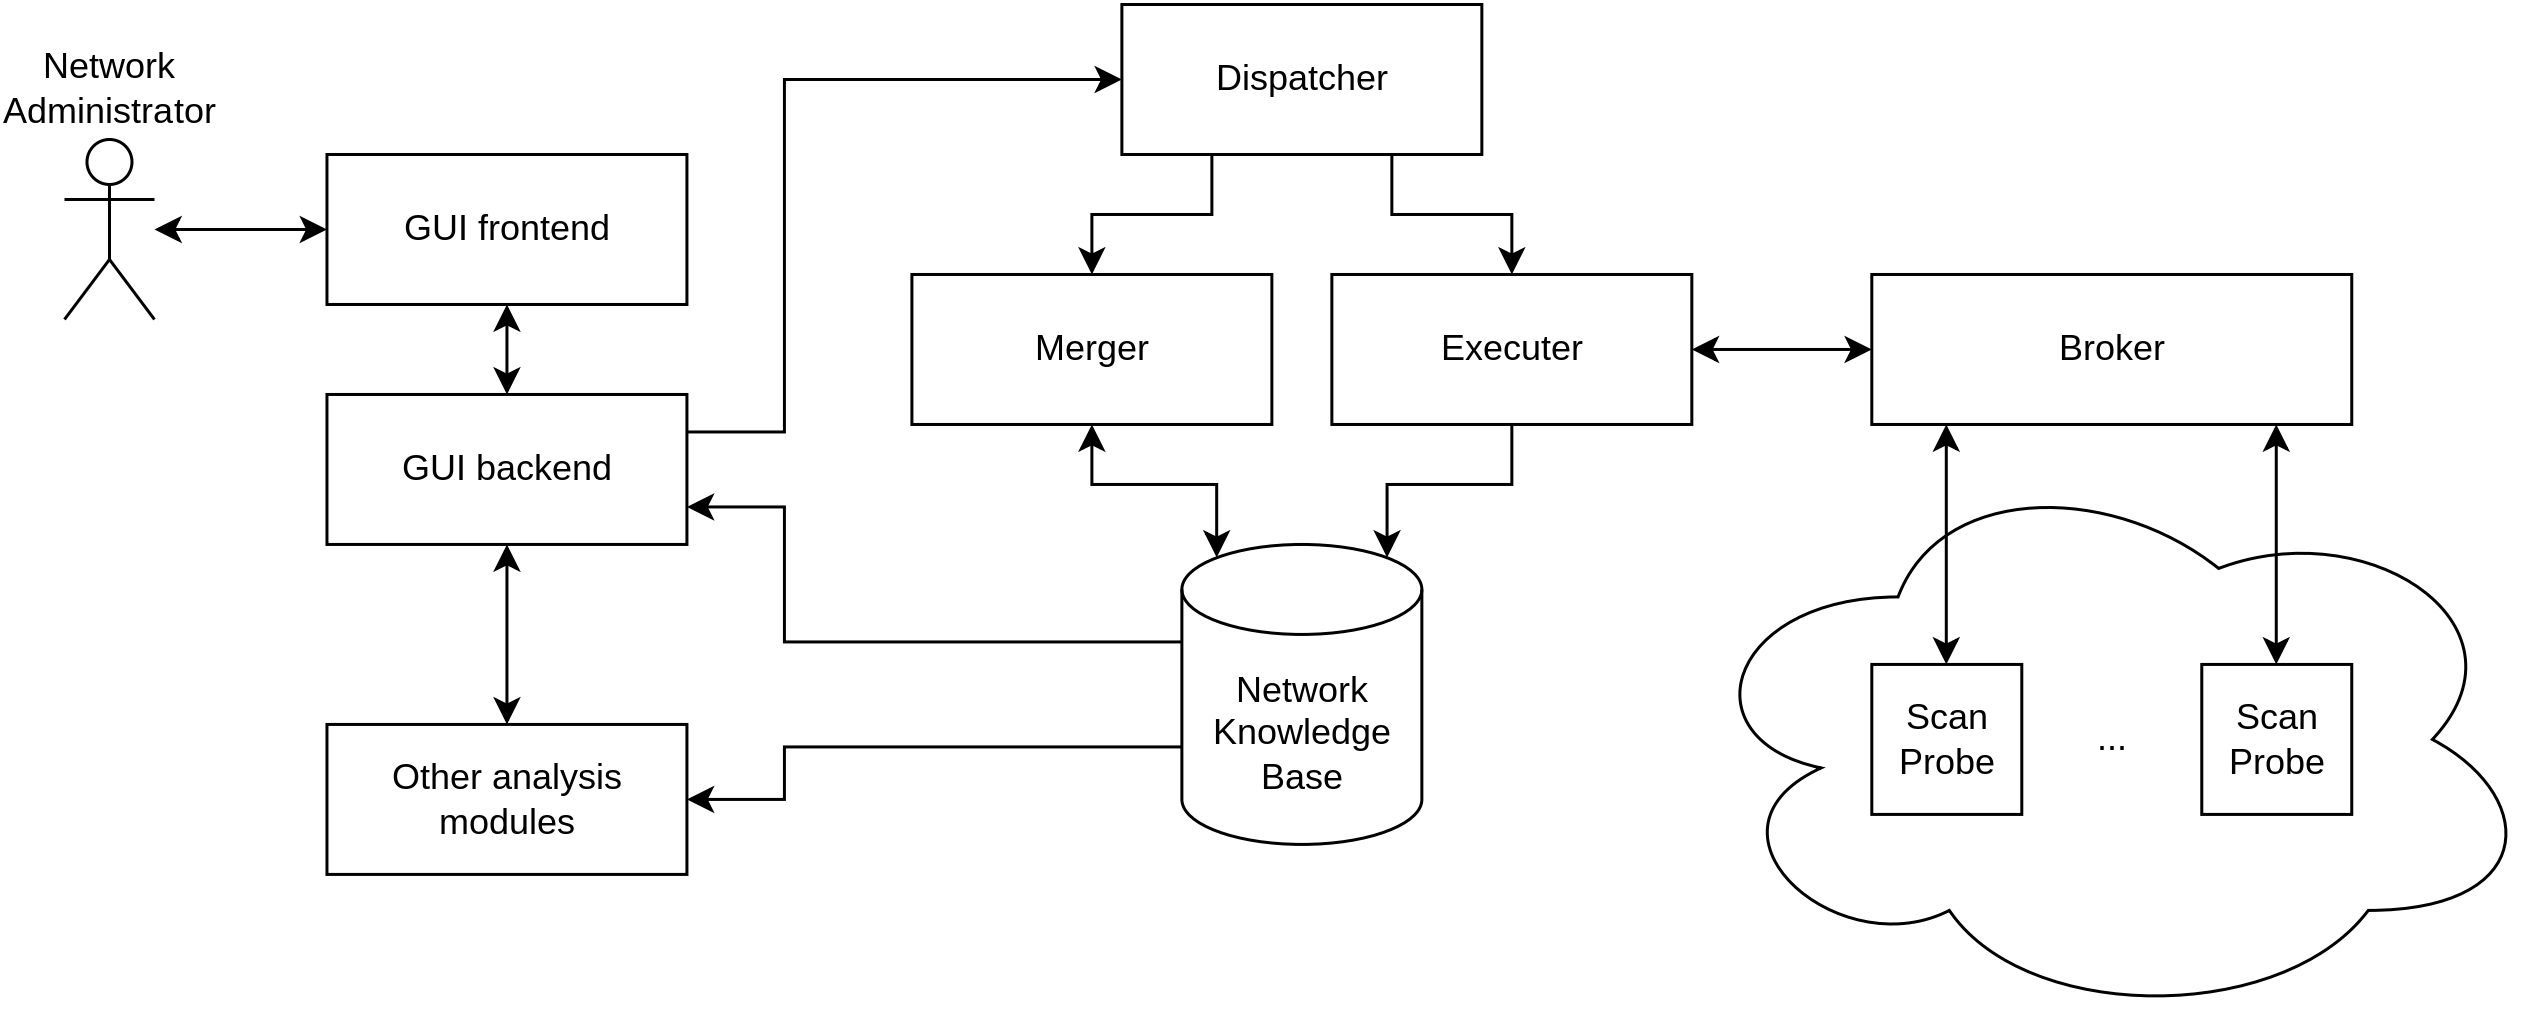
\includegraphics[width=\columnwidth]{moduli}
  \centering
  \caption{Moduli Architettura}
  \label{moduli}
\end{figure}

\FloatBarrier

\subsubsection{Scan Probes}
La Figura 4.3 illustra la struttura interna di una Scan Probe, una componente chiave del sistema distribuito che esegue le scansioni della rete target. La Scan Probe è composta da quattro moduli principali:
\begin{itemize}
  \item \textbf{Broker Communicator}: Questo modulo gestisce la comunicazione tra la Scan Probe e il Broker centrale. Riceve comandi dal Broker e invia i risultati delle scansioni completate. Il Broker Communicator agisce come l'interfaccia esterna della sonda, assicurando che tutte le istruzioni e i dati siano trasmessi correttamente tramite un protocollo di messaggistica (come MQTT).

  \item \textbf{Command Interpreter}: Una volta ricevuto un comando dal Broker Communicator, il Command Interpreter lo interpreta e lo trasforma in istruzioni eseguibili dal Scanner. Questo modulo è responsabile di tradurre i messaggi in azioni di scansione concrete, come eseguire una scansione specifica su una porzione di rete.

  \item \textbf{Scanner}: Il modulo Scanner è quello che esegue effettivamente la scansione della rete target, utilizzando strumenti come Nmap per raccogliere informazioni su dispositivi, porte, e servizi attivi all'interno della rete. I risultati della scansione vengono poi inviati al Formatter per essere elaborati e formattati correttamente.

  \item \textbf{Formatter}: Il modulo Formatter prende i dati raccolti dal Scanner e li organizza in un formato standard e comprensibile, pronto per essere inviato nuovamente al Broker Communicator. Questo step di formattazione è essenziale per assicurare che i risultati delle scansioni possano essere facilmente interpretati e utilizzati dagli altri moduli del sistema, come il Merger e la Knowledge Base.

\end{itemize}
In sintesi, la Scan Probe riceve comandi dal Broker, esegue le scansioni sulla rete target e restituisce i risultati in modo organizzato, consentendo al sistema di avere una visione aggiornata della rete in analisi.


\begin{figure}[t]
  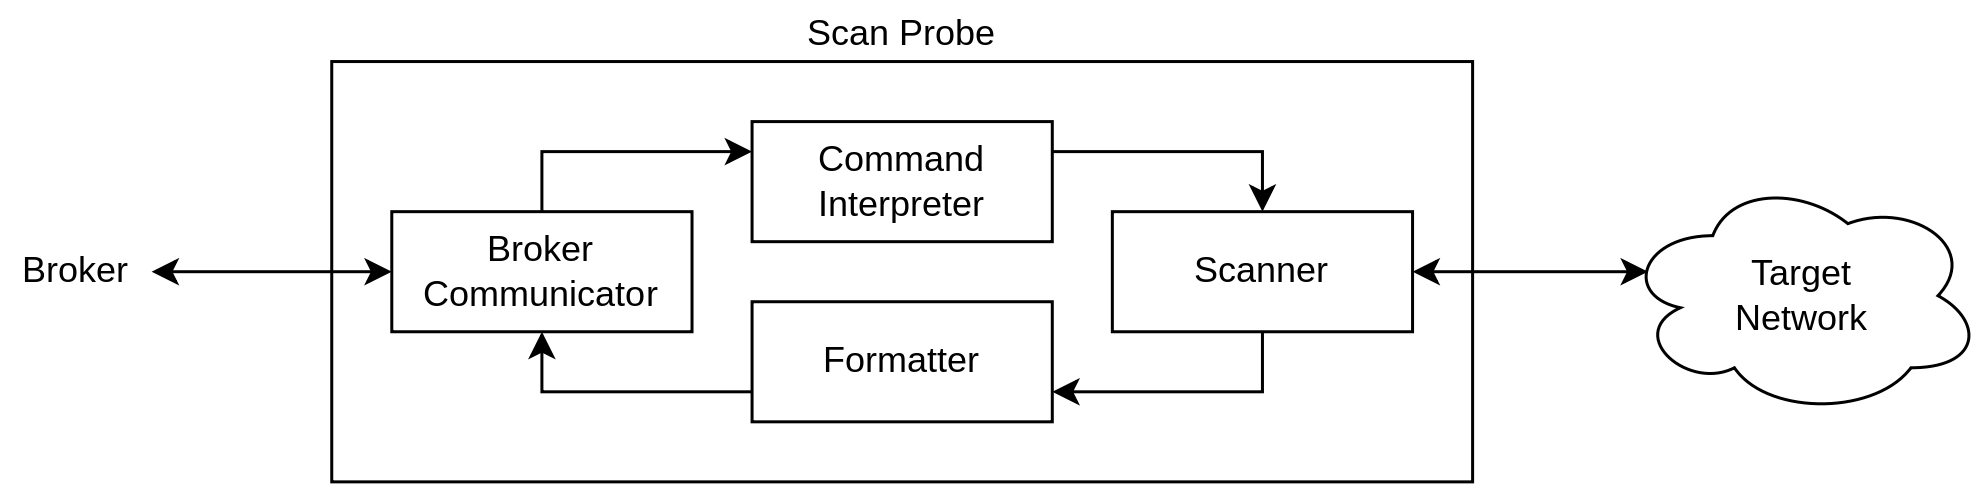
\includegraphics[width=\columnwidth]{probe}
  \centering
  \caption{Probe}
  \label{probe}
\end{figure}
\FloatBarrier


\subsubsection{Dispatcher} 
Il diagramma 4.4 rappresenta il funzionamento interno del Dispatcher, un componente fondamentale che gestisce la comunicazione tra la GUI e gli altri moduli del sistema, in particolare l'Executer e il Merger.

\begin{itemize}
  \item \textbf{GUI Communicator}: Questo modulo si occupa della comunicazione tra la GUI e il Dispatcher. Riceve i comandi dagli utenti attraverso l'interfaccia grafica e li invia al GUI Command Interpreter per l'elaborazione.

  \item \textbf{GUI Command Interpreter}: Una volta ricevuti i comandi dalla GUI, il GUI Command Interpreter li interpreta e li traduce in istruzioni comprensibili per il resto del sistema. Questa componente agisce come traduttore tra l'interfaccia utente e i processi interni del Dispatcher.

  \item \textbf{Scheduler}: Lo Scheduler prende le istruzioni dal GUI Command Interpreter e le organizza temporalmente, decidendo quando e come eseguire le azioni richieste. In pratica, stabilisce l'ordine e la priorità delle operazioni, gestendo le risorse disponibili.

  \item \textbf{Executer Communicator}: Dopo la schedulazione, lo Scheduler comunica le istruzioni programmate all'Executer tramite questo modulo. Questo canale garantisce che il Dispatcher possa inviare correttamente i comandi al modulo che esegue le scansioni.

  \item \textbf{Merger Communicator}: Infine, il Merger Communicator gestisce la comunicazione con il modulo Merger, inviando i dati necessari per la fusione dei risultati delle scansioni o altre informazioni elaborate. In questo modo, il Dispatcher collega direttamente i moduli di esecuzione delle scansioni e di gestione dei risultati.
\end{itemize}

il Dispatcher quindi è responsabile dell'interpretazione dei comandi dalla GUI, della loro programmazione e della gestione della comunicazione tra i vari moduli del sistema per garantire che le operazioni di scansione e fusione siano eseguite in modo efficiente e coordinato.

\begin{figure}[t]
  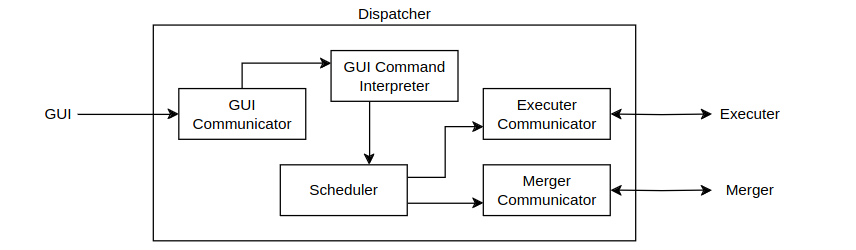
\includegraphics[width=\columnwidth]{dispatcher}
  \centering
  \caption{Dispatcher}
  \label{dispatcher}
\end{figure}

\FloatBarrier

\subsubsection{Executer} 
L'Executer (Figura 4.5) riceve un comando dallo Scheduler e coordina gli Scan Probes nell'esecuzione della scansione tramite un broker di messaggi idoneo. I risultati delle scansioni vengono poi salvati nel Network Knowledge Base.
\begin{itemize}
  \item \textbf{Dispatcher Communicator}: Riceve ordini dal Dispatcher che vengono interpretati ed inviati al supervisor.

  \item \textbf{Supervisor}: Gestisce i Probe e decide come suddividere il lavoro fra di loro. 

  \item \textbf{Broker Communicator}: Inoltra gli ordini dal Supervisor ai Probe e riceve i loro risultati ed eventuali altre informazioni tramite un Broker di messaggi.

  \item \textbf{Collector}: Raccoglie i messaggi dei Probe dal Broker Communicator, invia delle informazioni al Supervisor e invia i risultati delle scansioni al Knowledge Base Connector.

  \item \textbf{Knowledge Base Connector}: Riceve i dati delle scansioni e li invia alla Knowledge Base.
\end{itemize}

L'Executer in breve riceve i comandi dallo Scheduler e ordina ai singoli Probe di eseguire le scansioni. I risultati delle scansioni poi vengono inviati alla Network Base tramite il corrispondente connector.

\begin{figure}[t]
  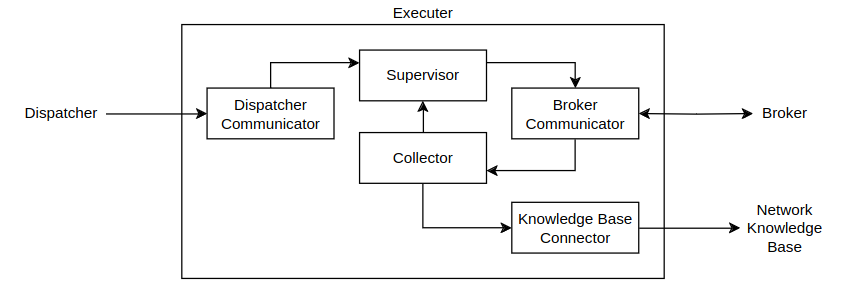
\includegraphics[width=\columnwidth]{executer}
  \centering
  \caption{Executer}
  \label{executer}
\end{figure}

\FloatBarrier

%/newpage

\subsubsection{Network Knowledge Base} 
Il modulo del Network Knowledge Base rappresenta il cuore del sistema di archiviazione e gestione dei dati raccolti dalle varie operazioni di scansione. La sua funzione principale è immagazzinare in modo sicuro e organizzato tutte le informazioni rilevanti sulla rete, come i risultati delle scansioni, i dettagli dei dispositivi rilevati, e altre metriche o log generati durante le attività di monitoraggio.

\FloatBarrier

\subsubsection{Merger}
Il Merger, rappresentato nella Figura 4.6, è una componente fondamentale del sistema che si occupa di raccogliere e unire i dati ottenuti dalle varie Scan Probe per fornire una visione completa e coerente della rete analizzata. Il suo scopo principale è quello di amalgamare i risultati delle scansioni provenienti da più sorgenti in una singola rappresentazione che permetta di comprendere lo stato complessivo della rete.
\begin{itemize}
  \item \textbf{Dispatcher Communicator}: Questo modulo ha il compito di ricevere comandi dal Dispatcher. I comandi che arrivano al Dispatcher Communicator vengono trasmessi al modulo successivo per essere interpretati e gestiti.

  \item \textbf{Command Interpreter}: Come suggerisce il nome, il Command Interpreter è responsabile dell'interpretazione dei comandi ricevuti dal Dispatcher Communicator. Questo modulo verifica che i comandi siano corretti, li decodifica e determina quale operazione deve essere eseguita dall'Amalgamator. L'interpretazione precisa dei comandi è cruciale per garantire che il processo di aggregazione dei dati avvenga correttamente e nel giusto contesto operativo. 

  \item \textbf{Amalgamator}: Il cuore del Merger, l'Amalgamator, è la componente che esegue l'effettiva amalgamazione dei dati. Una volta ricevuto un comando dal Command Interpreter, l'Amalgamator si connette al Knowledge Base Connector per recuperare tutti i dati necessari per generare una mappa aggiornata e comprensibile della rete. Questo processo di aggregazione utilizza un algoritmo che integra e sintetizza le informazioni provenienti dalle diverse scansioni, eliminando duplicazioni o discrepanze e creando una rappresentazione coerente. L'obiettivo finale è produrre un'istantanea della rete che riflette accuratamente lo stato attuale delle connessioni, dei dispositivi e delle eventuali vulnerabilità.

  \item \textbf{Knowledge Base Connector}: Agisce come intermediario tra l'Amalgamator e il Network Knowledge Base. Si occupa di fornire all'Amalgamator tutti i dati necessari per l'aggregazione e successivamente di salvare le mappe di rete generate nel Knowledge Base per una consultazione futura. Grazie a questa componente, il Merger può interagire dinamicamente con il database e ottenere accesso rapido alle informazioni più aggiornate, garantendo che i dati utilizzati per l'amalgamazione siano sempre accurati e pertinenti.
\end{itemize}


\begin{figure}[t]
  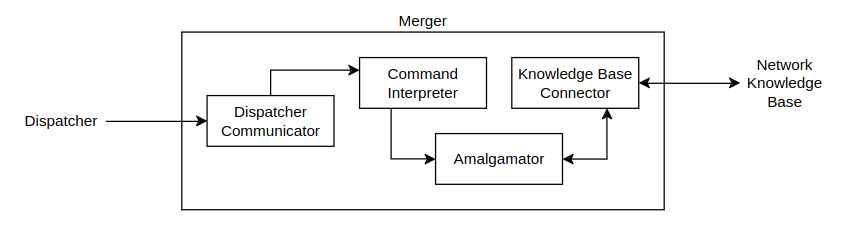
\includegraphics[width=\columnwidth]{merger}
  \centering
  \caption{Merger}
  \label{merger}
\end{figure}

\FloatBarrier


\subsubsection{GUI} 
Il modulo della GUI (Graphical User Interface) è l'interfaccia utente del sistema, che consente agli amministratori di rete di interagire in modo intuitivo con le funzionalità del sistema. Attraverso la GUI, è possibile inviare comandi, visualizzare i risultati delle scansioni, monitorare lo stato della rete e gestire altre operazioni chiave senza dover interagire direttamente con i componenti backend.

La GUI è composta da due parti principali:

\begin{itemize}
  \item \textbf{GUI Frontend}: L'interfaccia grafica vera e propria, visualizzata sullo schermo e utilizzata dagli utenti per inviare input, come richieste di scansione o richieste di visualizzazione della rete.
  \item \textbf{GUI Backend}: Il modulo che si occupa della logica di elaborazione e della gestione delle richieste utente, interfacciandosi con il resto del sistema tramite il Dispatcher.
\end{itemize}

la GUI rende il sistema accessibile e facile da utilizzare, permettendo un controllo visivo e immediato della rete e delle operazioni in corso.

\FloatBarrier

%\chapter{In Dettaglio: Executer}
\chapter{Il modulo Executer}
In questo capitolo viene descritto in dettaglio il funzionamento dell'executer che, come spiegato in breve nel capitolo prima, funge da componente centrale per la gestione della comunicazione e della supervisione delle attività all'interno del sistema.


\section{Dispatcher Communicator}
Il Dispatcher Communicator è il componente responsabile di ricevere comandi o dati dal modulo Dispatcher esterno. Il Dispatcher è un'entità centrale che invia istruzioni al Executer all'interno del sistema distribuito, fungendo da orchestratore. Il ruolo principale del Dispatcher Communicator è quello di stabilire una connessione stabile e affidabile con il Dispatcher e garantire che i messaggi inviati vengano processati correttamente. Una volta ricevuti i dati, il Dispatcher Communicator passa l'informazione al Supervisor per ulteriori azioni.
Oltre alla ricezione, il Dispatcher Communicator dovrebbe anche gestire l'eventuale feedback o risposta da inviare al Dispatcher, ad esempio conferme di esecuzione o report di stato. In scenari di reti distribuite su larga scala, il Dispatcher Communicator deve garantire che i messaggi siano consegnati anche in condizioni di rete congestionata o instabile. A tal fine, nell'implementazione  abbiamo utilizzando protocolli di rete affidabili come MQTT che verranno descritti nel capitolo successivo. L'efficacia di questo componente è cruciale per mantenere la sincronia e l'affidabilità del sistema, poiché è il punto di ingresso primario per le richieste di esecuzione di task.


\section{Supervisor}
Il Supervisor è il componente centrale dell'Executer che coordina e supervisiona l'esecuzione delle varie operazioni. Agisce come un gestore dei task, ricevendo input dal Dispatcher Communicator e determinando come e quando delegare i compiti agli altri moduli interni dell'Executer. Il Supervisor decide quali azioni intraprendere in base ai dati ricevuti e alle informazioni raccolte all'interno del sistema, interagendo costantemente con gli altri componenti come il Broker Communicator e il Collector.
Il Supervisor svolge un ruolo fondamentale nel garantire che le risorse vengano allocate correttamente e che i flussi di lavoro seguano un percorso ottimale. Può anche implementare logiche di fault-tolerance, monitorando lo stato delle varie parti del sistema e intervenendo in caso di malfunzionamenti. Inoltre, il Supervisor è responsabile di gestire la concorrenza tra task, assicurando che più operazioni possano essere eseguite in parallelo senza interferenze o colli di bottiglia. In un'architettura distribuita, il Supervisor deve essere altamente reattivo e scalabile, capace di orchestrare task in tempo reale e mantenere un alto grado di coerenza e integrità dei dati.

\section{Broker Communicator}
Il Broker Communicator gestisce la comunicazione tra l'Executer e un modulo esterno denominato Broker. Il Broker è un middleware che facilita lo scambio di messaggi tra i vari componenti di un sistema distribuito, e può utilizzare protocolli come MQTT, Kafka \cite{kreps2015kafka} o altri sistemi di messaggistica. Il ruolo del Broker Communicator è quello di inviare e ricevere dati dal Broker, garantendo che i messaggi siano consegnati in modo affidabile e che le informazioni siano correttamente inoltrate tra i componenti del sistema.
Il Broker Communicator deve gestire più canali di comunicazione contemporaneamente, inviando messaggi a diversi destinatari e ricevendo dati da più fonti. In scenari di monitoraggio e analisi della rete. Una delle principali sfide affrontate dal Broker Communicator è garantire che i messaggi siano consegnati in maniera affidabile e senza perdita di dati, anche in ambienti di rete instabili. 

\section{Collector}
Il Collector è il componente che si occupa della raccolta e aggregazione dei dati all'interno del sistema. Riceve le informazioni dal Broker Communicator e la sua funzione principale è quella di raccogliere, filtrare e organizzare i dati che saranno poi utilizzati per aggiornare la Network Knowledge Base attraverso il Knowledge Base Connector.
Il Collector potrebbe avere la capacità di analizzare i dati raccolti in tempo reale, aggregarli, trasformarli in un formato standardizzato e fornire insight utili al Supervisor come il termine di una scansione. Inoltre, potrebbe essere responsabile della gestione delle metriche di performance e dello stato della rete. In sistemi di rete complessi, il Collector deve essere in grado di elaborare grandi quantità di dati in maniera efficiente, assicurandosi che la latenza sia ridotta al minimo. La sua scalabilità è critica in ambienti di rete di grandi dimensioni, poiché deve gestire un flusso continuo di dati provenienti da diverse fonti distribuite.

\section{Knowledge Base Connector}
l Knowledge Base Connector è il modulo che interfaccia l'Executer con una Network Knowledge Base esterna, il cui scopo è raccogliere e mantenere la conoscenza relativa alla topologia della rete, alle metriche di performance e ad altri dati critici. Questo componente funge da ponte tra il sistema distribuito e la base di conoscenza, permettendo al sistema di aggiornare continuamente il database con nuove informazioni ottenute dal Collector.
Il Knowledge Base Connector potrebbe inviare dati strutturati, come informazioni sui nodi e sui dispositivi della rete, configurazioni, e statistiche sulle performance, alla Knowledge Base. Per garantire l'affidabilità, potrebbe utilizzare protocolli di rete sicuri e meccanismi di autenticazione per proteggere i dati sensibili. In un sistema distribuito complesso, è essenziale che il Knowledge Base Connector garantisca l'accuratezza e la tempestività degli aggiornamenti, poiché la Knowledge Base funge da risorsa centrale per l'analisi della rete e la previsione di problemi futuri.

%\chapter{Implementazione Executer}
\chapter{Implementazione del modulo Executer}
In questo capitolo verranno descritte in dettaglio le scelte di implementazione adottate per i vari sottomoduli dell'Executer, illustrando come ciascuna componente è stata progettata per garantire una comunicazione efficiente e un'operatività ottimale all'interno del sistema distribuito.
Di seguito le soluzioni tecniche adottate, le librerie e gli strumenti utilizzati, nonché le motivazioni alla base di tali scelte, con particolare attenzione all'efficienza, scalabilità e modularità del sistema.

\section{Comunicazione interna}
I sottomoduli dell'Executer comunicano fra loro direttamente all'interno del linguaggio Rust utilizzando il meccanismo di comunicazione basato su canali, fornito dalla libreria standard tramite il modulo std::sync::mpsc \cite{rust_mpsc}. Questo approccio permette la trasmissione di messaggi tra componenti in modo sicuro e asincrono, evitando condizioni di gara e garantendo un flusso ordinato di dati.
\subsection{std::sync::mpsc}
mpsc sta per multi-producer, single-consumer. Questo significa che più produttori (sorgenti di dati) possono inviare messaggi su un canale verso un unico consumatore (ricevitore). Ogni sottomodulo dell'Executer che deve inviare dati a un altro modulo agisce come produttore, mentre il destinatario agisce come consumatore.
Un canale è un concetto utilizzato per trasmettere dati o messaggi tra diverse parti di un programma tra tra thread che definiscono i sottomoduli. Rust implementa i canali con due entità principali:

\begin{itemize}
  \item Sender: Lato del produttore del canale. Qualsiasi sottomodulo che deve inviare dati ad altri moduli utilizza un'istanza di Sender.
  \item Receiver: Lato del consumatore. Il modulo che riceve i messaggi avrà un'istanza di Receiver.
\end{itemize}
FIFO (First In, First Out): La coda che gestisce i messaggi all'interno del canale segue la politica FIFO. Ciò significa che i messaggi vengono ricevuti nell'ordine in cui sono stati inviati, garantendo che i dati siano elaborati in modo sequenziale e prevedibile. Questo è particolarmente importante in un contesto distribuito, dove l'ordine delle operazioni può influenzare l'integrità del sistema.
\subsection{Vantaggi di mpsc}
\textbf{Sicurezza concorrente}: Utilizzando mpsc, si evita l'uso di memoria condivisa o accessi simultanei alle stesse risorse da parte di più thread. Ogni modulo comunica tramite messaggi, mantenendo l'isolamento dei dati e prevenendo deadlock o race conditions, che potrebbero compromettere la correttezza del sistema. 
\newline
\textbf{Asincronia}: I canali sono non bloccanti, quindi il modulo produttore può continuare a funzionare anche dopo aver inviato un messaggio, senza doversi preoccupare se il messaggio sia stato già ricevuto o elaborato. Il modulo consumatore, invece, può leggere i messaggi appena necessario.
\newline
\textbf{Scalabilità}: La capacità di avere più produttori garantisce che il sistema possa scalare facilmente aggiungendo nuovi componenti che inviano dati su un singolo canale, senza dover cambiare la logica del consumatore.
\subsection{Utilizzo nell'Executer}
In questo contesto, ogni sottomodulo dell'Executer (come il Supervisor, il Dispatcher Communicator, il Broker Communicator, etc.) funge da produttore o consumatore, a seconda del flusso di comunicazione richiesto. Ad esempio il Dispatcher Communicator può inviare comandi al Supervisor attraverso un canale.

Questo schema di comunicazione rende il sistema modulare e facile da estendere, poiché ogni modulo è indipendente dagli altri e può essere collegato a più sottomoduli tramite semplici meccanismi di invio e ricezione di messaggi.

\section{Comunicazione esterna}
All'interno dell'architettura dell'Executer, i vari sottomoduli comunicano fra loro utilizzando rust ma per la comunicazione fra diversi moduli, quindi ad esempio la comunicazione fra Executer e Dispatcher, viene usato il protocollo MQTT (Message Queuing Telemtry Transport), un protocollo di messaggistica leggero e asincrono, particolarmente adatto per ambienti distribuiti e reti connesse. Come broker MQTT, viene utilizzato Mosquitto, un'implementazione open-source ampiamente diffusa e affidabile. 
\subsection{Cos'è MQTT?}
MQTT \cite{mqtt2024} è un protocollo di messaggistica basato sul paradigma publish/subscribe. Invece di inviare messaggi direttamente tra un mittente e un destinatario, come nei tradizionali modelli point-to-point, MQTT opera attraverso un broker centrale che gestisce la comunicazione tra i vari partecipanti al sistema.
\begin{itemize}
  \item \textbf{Publish/Subscribe}: I moduli del sistema non comunicano direttamente tra loro, ma attraverso argomenti (topics). Un modulo pubblica messaggi su un determinato topic e uno o più moduli che si sono iscritti (subscribed) a quel topic ricevono il messaggio. Questo permette una comunicazione altamente decoupled, dove i moduli non hanno bisogno di conoscere direttamente gli altri moduli con cui comunicano.
  \item \textbf{Asincrono e leggero}: MQTT è progettato per essere leggero, ideale per reti a larghezza di banda limitata o dispositivi con capacità ridotte. La comunicazione è asincrona, quindi i moduli possono inviare e ricevere messaggi senza bloccare le proprie operazioni, favorendo la scalabilità.
  \item \textbf{Qualità del servizio (QoS)}: MQTT offre vari livelli di garanzia sulla consegna dei messaggi, permettendo di scegliere tra una semplice "fire-and-forget" (livello 0), conferma di ricezione (livello 1), o consegna garantita esattamente una volta (livello 2). Questa flessibilità consente di bilanciare affidabilità e prestazioni a seconda dei requisiti del sistema.
\end{itemize}

\subsection{Cos'è Mosquitto?}
Mosquitto \cite{mosquitto2024} è un'implementazione open-source del broker MQTT, che funge da intermediario per la comunicazione tra i vari moduli del sistema. È responsabile della gestione degli argomenti e della distribuzione dei messaggi ai moduli corretti, in base agli argomenti a cui sono iscritti.
\begin{itemize}
  \item \textbf{Broker}: Un broker MQTT come Mosquitto è l'elemento centrale in una rete MQTT. Tutti i messaggi passano attraverso di esso, e ha il compito di distribuire i messaggi dai publisher agli abbonati in modo efficiente. Il broker si occupa anche di mantenere le connessioni attive e gestire eventuali riconnessioni in caso di interruzioni.
  \item \textbf{Efficienza e scalabilità}: Mosquitto è progettato per essere leggero e può gestire un gran numero di connessioni simultanee con un consumo minimo di risorse, il che lo rende ideale per l'utilizzo in reti distribuite come quella dell'Executer. Inoltre, Mosquitto supporta sia connessioni con autenticazione che connessioni criptate, garantendo un alto livello di sicurezza per le comunicazioni tra moduli.
\end{itemize}


\section{Supervisor}
Il Supervisor, per svolgere correttamente il suo ruolo, deve avere una visione aggiornata di tutti i Probe attivi nel sistema. Ogni volta che un nuovo Probe si registra, invia un messaggio di registrazione tramite il protocollo MQTT. Questo messaggio, pubblicato su un topic specifico a cui l'Executer è iscritto, contiene un Probe ID univoco, che identifica il probe all'interno della rete.

Il Supervisor riceve il messaggio e, successivamente, memorizza l'ID del probe in una struttura dati. Attualmente, abbiamo scelto di utilizzare una coda come struttura temporanea per facilitare l'implementazione dell'algoritmo di bilanciamento del carico (load balancing). L'algoritmo scelto per la prima fase è il Round Robin , un metodo semplice e equo che garantisce a ogni probe registrato di ricevere incarichi in modo sequenziale, evitando la predominanza di uno rispetto agli altri.

Tuttavia, in futuro, sarà necessario adottare un approccio più avanzato per il bilanciamento del carico, che tenga conto delle dimensioni e della complessità delle reti gestite da ciascun Probe. Un possibile miglioramento prevede l'introduzione di una priorità associata ai probe che gestiscono porzioni più estese della rete, sempre garantendo che nessun probe venga trascurato o si trovi in condizione di starvation. Questo approccio permetterebbe una distribuzione più efficiente e dinamica dei compiti, bilanciando meglio il carico di lavoro tra i vari componenti del sistema.

\section{Broker Communicator}
Il Broker Communicator è responsabile dello scambio di messaggi con il broker MQTT, Mosquitto, gestendo sia l'invio che la ricezione delle comunicazioni all'interno del sistema distribuito. Le interazioni avvengono principalmente in due direzioni:
\newline
\textbf{Invio dei messaggi}: Quando il Supervisor richiede una scansione, il Broker Communicator si occupa di incorporare la richiesta all'interno di un messaggio MQTT strutturato e di pubblicarlo sul topic appropriato, che verrà poi processato dai vari probe registrati. Questo meccanismo garantisce che la richiesta raggiunga i destinatari in modo asincrono ed efficiente.
\newline
\textbf{Ricezione dei messaggi}: La ricezione dei messaggi da parte del Broker Communicator è suddivisa in tre principali categorie:
\begin{itemize}

  \item \textbf{Register}: Questi messaggi sono inviati dai probe per notificare la loro iscrizione al sistema. Ogni nuovo probe, al momento della registrazione, invia un messaggio contenente il suo identificativo univoco (Probe ID), permettendo così al sistema di tenerne traccia.

  \item \textbf{Result}: Dopo aver completato una scansione, i probe inviano i risultati al sistema sotto forma di messaggi Result. Questi includono tutte le informazioni raccolte durante la scansione, che vengono poi elaborate dal Supervisor o da altri componenti del sistema.

  \item \textbf{Info}: Questa categoria di messaggi include informazioni aggiuntive relative allo stato delle scansioni, come eventuali errori riscontrati o altri dati utili per il monitoraggio e il debug del sistema.
\end{itemize}

Grazie a questa architettura, il Broker Communicator garantisce una comunicazione fluida e coordinata tra i vari componenti del sistema, mantenendo l'interoperabilità tra probe e Supervisor tramite Mosquitto.

\section{Collector}
Questo modulo è progettato per ricevere messaggi dal Broker Communicator attraverso un canale mpsc (multi-producer, single-consumer). Il funzionamento del Collector è basato sul tipo di messaggio ricevuto, che viene processato in modo differente a seconda del suo contenuto.

Attualmente, il Collector gestisce i messaggi in questo modo:
\begin{itemize}
  \item \textbf{Messaggi di registrazione}: Se il messaggio ricevuto riguarda la registrazione di un Probe, il Collector estrae l'ID del probe e lo invia al Supervisor utilizzando l'apposito canale mpsc configurato per la comunicazione interna.

  \item \textbf{Messaggi di risultati}: Quando viene ricevuto un messaggio contenente i risultati di una scansione effettuata da un probe, il Collector inoltra questi dati al Knowledge Base Connector, che si occupa di integrarli nel sistema di conoscenza della rete.

  \item \textbf{Messaggi di info}: Per i messaggi di tipo informativo, come errori o aggiornamenti sullo stato delle scansioni, il Collector li trasmette anch'essi al Knowledge Base Connector per permettere un monitoraggio più accurato dello stato del sistema.
\end{itemize}

Nel futuro, sarà importante migliorare il sistema di filtraggio dei dati che il Collector elabora, garantendo comunque che la latenza rimanga il più bassa possibile. Questo permetterà di ottimizzare le prestazioni del sistema, soprattutto in ambienti di rete molto dinamici o in caso di elevato traffico di messaggi.

\section{Dispatcher Communicator}
Per l'implementazione del Dispatcher Communicator, dato che il modulo del dispatcher non è ancora stato implementato, al momento utilizziamo una simulazione basata su MQTT per la gestione della comunicazione tra i moduli. Questa simulazione ci permette di testare l'invio e la ricezione dei messaggi in modo realistico, utilizzando il broker Mosquitto per replicare il comportamento previsto del dispatcher.

In questo modo, possiamo procedere con lo sviluppo e la verifica del sistema, garantendo che i flussi di comunicazione siano correttamente gestiti e mantenendo flessibilità nell'evoluzione dell'architettura. L'integrazione del dispatcher effettivo verrà eseguita in futuro, sostituendo progressivamente la simulazione con l'implementazione finale.

\section{Knowledge Base Connector}
Il Knowledge Base Connector è una componente essenziale per l'architettura del sistema, progettata per gestire tutte le interazioni con il database da parte dell'Executer. La sua implementazione in Rust è stata pensata per essere modulare e flessibile, consentendo al sistema di archiviare e aggiornare informazioni sulla topologia di rete in modo efficiente e scalabile.

\subsection{Connessione a ScyllaDB}
Il database scelto per l’implementazione del Knowledge Base Connector è ScyllaDB \cite{scylladb2024}, un database NoSQL altamente scalabile, basato su una tecnologia compatibile con Cassandra \cite{cassandra2024}, ma ottimizzato per prestazioni superiori. La scelta di ScyllaDB si basa sulla sua capacità di gestire grandi quantità di dati distribuiti su più nodi, con bassa latenza e alta efficienza, requisiti fondamentali per un sistema distribuito che analizza una rete su larga scala.

\subsection{Supporto JSON ScyllaDB}
Uno dei vantaggi principali di ScyllaDB è il suo supporto nativo per il formato JSON. Questa funzionalità ci permette di memorizzare strutture di dati complesse in modo flessibile all'interno delle tabelle del database, mantenendo la struttura gerarchica dei dati senza la necessità di mappare ogni campo singolarmente in colonne tradizionali. Utilizzare JSON permette di avere un formato molto adatto a rappresentare i risultati delle scansioni di rete, che possono includere dettagli come indirizzi IP, porte aperte, protocolli e altre informazioni correlate alla topologia di rete.

La scelta di utilizzare il supporto JSON semplifica enormemente la gestione dei dati in quanto permette di inserire e recuperare oggetti complessi senza doverli disaggregare, migliorando così l'efficienza e riducendo la complessità delle query.

\subsection{Interacce modulari}
Per facilitare eventuali cambiamenti futuri nel database, l’implementazione del Knowledge Base Connector è stata costruita utilizzando interfacce modulari. Questo design consente al sistema di interagire con il database tramite un livello di astrazione che separa la logica dell'applicazione dai dettagli specifici del database scelto.

Grazie a questa struttura, è possibile sostituire ScyllaDB con un altro sistema di database, come PostgreSQL \cite{postgresql2024} o MongoDB \cite{mongodb2024}, con modifiche minime al codice. Il livello di astrazione garantisce che le operazioni principali come l’inserimento rimangano invariate, indipendentemente dal tipo di database sottostante.

\subsection{Funzionamento Knowledge Base Connector}
Il Knowledge Base Connector svolge diverse operazioni cruciali:

\begin{itemize}
  \item \textbf{Inserimento dei risultati delle scansioni}: Quando un Probe invia i risultati di una scansione, il Collector inoltra questi dati al Knowledge Base Connector. Questi dati, strutturati in formato JSON, vengono memorizzati in ScyllaDB tramite query appositamente create per gestire il formato JSON. Questo approccio permette di preservare la complessità e l'integrità delle informazioni senza necessità di trasformazioni complesse.
  \item \textbf{Aggiornamento della topologia di rete}: Il sistema è progettato per eseguire aggiornamenti incrementali della topologia di rete. Man mano che arrivano nuove informazioni dai Probe, il Knowledge Base Connector aggiorna le entità esistenti nel database. Grazie alla flessibilità del formato JSON, è possibile modificare solo alcune parti dei dati senza dover riscrivere interamente un record, migliorando l'efficienza e riducendo la latenza delle operazioni di scrittura.
  \item \textbf{Gestione delle query}: Per garantire che le prestazioni rimangano elevate anche in presenza di grandi volumi di dati, le query verso ScyllaDB sono state ottimizzate. La struttura a interfacce modulari permette di aggiungere o modificare facilmente query più avanzate per soddisfare requisiti futuri senza cambiare l'architettura di base del sistema.
\end{itemize}



\subsection{Vantaggi Modularità}
La modularità offerta dall'utilizzo delle interfacce ha diversi vantaggi. Prima di tutto, permette una facile sostituzione del database qualora ScyllaDB non fosse più adeguato o se emergessero nuovi requisiti. Inoltre, questo approccio facilita l’aggiunta di nuove funzionalità legate alla gestione dei dati, come l’integrazione con motori di ricerca distribuiti o la possibilità di archiviare diversi tipi di dati in base a contesti specifici.

Infine, la modularità facilita anche lo sviluppo e la manutenzione del sistema nel lungo termine. Con un design che non è strettamente legato a ScyllaDB, gli sviluppatori possono continuare a evolvere il sistema mantenendo separata la logica applicativa dal livello di persistenza dei dati, rendendo l'intero sistema più flessibile e manutenibile.

\subsection{Conclusione}
L'implementazione del Knowledge Base Connector si fonda su principi di modularità, flessibilità e prestazioni. La scelta di ScyllaDB, con il suo supporto nativo per JSON, offre un'ottima base per gestire i dati complessi derivanti dalle scansioni di rete, mentre l'uso di interfacce garantisce la facilità di adattamento a cambiamenti futuri nel sistema di database. Questi elementi consentono al sistema di crescere ed evolvere in modo sostenibile, mantenendo alte prestazioni e una gestione efficiente della topologia di rete.


\section{Altre librerie usate}
Nel progetto, oltre alle librerie già menzionate, sono state utilizzate diverse altre librerie di Rust che hanno giocato un ruolo fondamentale nell'implementazione delle varie componenti del sistema. Di seguito vengono descritte alcune delle principali librerie e il loro utilizzo:
\subsection{Anyhow}

La libreria anyhow \cite{rust_anyhow} viene utilizzata per la gestione degli errori. Rust fornisce un sistema di gestione degli errori molto rigoroso, e anyhow semplifica notevolmente il processo, permettendo di trattare gli errori in modo più flessibile, specialmente nei contesti in cui la precisione nel gestire ogni singola casistica non è strettamente necessaria.
\begin{itemize}
  \item \textbf{Gestione degli errori flessibile}: Anyhow permette di aggregare e gestire vari tipi di errori attraverso il tipo anyhow::Error, rendendo la scrittura del codice più semplice e mantenendo comunque la robustezza necessaria in un sistema distribuito.
  \item \textbf{Backtrace e Debugging}: Inoltre, anyhow fornisce strumenti per generare stack trace dettagliati, che sono molto utili durante il debugging, in modo da poter risalire velocemente alla causa di un errore.
\end{itemize}
In un sistema distribuito complesso come il nostro, in cui le comunicazioni tra moduli e il parsing dei dati devono essere sempre gestiti in modo corretto, anyhow facilita la cattura e la propagazione degli errori tra le varie componenti.

\subsection{Tracing}
La libreria tracing \cite{rust_tracing} è utilizzata per il logging strutturato e l'osservabilità del sistema. Diversamente dalle tradizionali librerie di logging, tracing permette di ottenere informazioni dettagliate sul comportamento del programma, fornendo uno strumento utile per monitorare in modo efficiente i flussi di esecuzione.
\begin{itemize}
  \item \textbf{Eventi e Span}: tracing introduce il concetto di span e eventi. Uno span rappresenta una singola operazione o funzione nel programma, e può essere nidificato o contenere altre operazioni all'interno. Gli eventi, invece, sono punti specifici che segnalano qualcosa di importante che accade nel programma. Questo modello risulta particolarmente utile per tracciare l'esecuzione asincrona, poiché rende possibile capire il contesto di esecuzione di una determinata operazione.
  \item \textbf{Logging avanzato}: Rispetto ad altre librerie di logging, tracing consente di raccogliere informazioni più dettagliate su ogni evento e su come si relaziona ad altre operazioni del sistema. Questo è particolarmente utile in ambienti distribuiti come il nostro, dove molte operazioni avvengono in parallelo e potrebbero essere difficili da tracciare correttamente.
\end{itemize}

Grazie a tracing, è possibile tenere sotto controllo lo stato di esecuzione dei vari moduli, tra cui l'Executer, monitorando le loro interazioni e migliorando l'osservabilità e il debugging del sistema.

\subsection{Tokio}
Tokio \cite{rust_tokio} è una delle librerie più utilizzate in Rust per la gestione della programmazione asincrona. Poiché il nostro sistema è distribuito e molte operazioni devono essere eseguite contemporaneamente o in modo asincrono, tokio è stata fondamentale per implementare efficientemente il modello asincrono.
\begin{itemize}
  \item \textbf{Runtime asincrono}: Tokio fornisce un runtime asincrono basato su un modello di event loop, che permette al sistema di gestire molte operazioni in parallelo senza bloccare i thread. Questo è essenziale per l'esecuzione di task come l'invio e la ricezione di messaggi MQTT o la gestione delle comunicazioni tra moduli, che richiedono di essere gestite contemporaneamente ma senza sovraccaricare il sistema.
  \item \textbf{Task e thread}: Tokio permette di creare task che possono essere eseguite su thread separati, bilanciando il carico di lavoro tra le diverse componenti del sistema in modo efficiente. È utilizzato nel nostro progetto per gestire le comunicazioni tra i vari moduli, permettendo loro di funzionare senza blocchi anche quando attendono nuovi messaggi o dati di input.
\end{itemize}

La scelta di Tokio è stata fondamentale per permettere al sistema di scalare, rendendo possibile la gestione di numerose connessioni simultanee senza compromettere le prestazioni.

\subsection{Serde}
La libreria serde \cite{rust_serde} è stata utilizzata per il serialization e deserialization dei dati, ovvero la conversione tra strutture di dati di Rust e formati esterni (come JSON o XML). Dato che il sistema comunica tramite protocolli che trasportano dati strutturati, serde è essenziale per poter convertire agevolmente questi dati da e verso i formati utilizzati nelle comunicazioni tra i moduli.
\begin{itemize}
  \item \textbf{Serializzazione/Deserializzazione}: Nel nostro progetto, serde viene utilizzata principalmente per il parsing dei dati XML ricevuti dai Probe. Consente di mappare facilmente i dati ricevuti in strutture Rust, semplificando l'analisi e la gestione delle informazioni all'interno del sistema.
  \item \textbf{Modularità e flessibilità}: Grazie alla sua architettura modulare, serde permette di supportare vari formati di dati, adattandosi facilmente ai diversi requisiti del sistema.
\end{itemize}

Grazie all'utilizzo di serde, il sistema può gestire con facilità formati di dati complessi e strutturati, migliorando l'integrazione e la gestione delle comunicazioni tra i moduli.



%% Capitolo
\chapter{Conclusioni}
In questa tesi è stato sviluppato e implementato il modulo \textbf{Executer}, che rappresenta una componente centrale nel sistema distribuito per l'analisi della topologia di reti di calcolatori. Il lavoro ha riguardato la gestione delle comunicazioni tra i vari moduli del sistema e il coordinamento delle operazioni di raccolta ed elaborazione dei dati di rete, sfruttando un'architettura a messaggistica distribuita. L'implementazione del modulo Executer è stata completata con successo, consentendo la ricezione, l'elaborazione e l'invio di comandi e risultati all'interno del sistema.

Sebbene durante lo sviluppo siano stati implementati anche altri moduli, come il \textbf{Probe}, che sarà descritto in un altro lavoro, rimangono da completare ulteriori componenti fondamentali. Tra questi, il \textbf{Dispatcher}, il \textbf{Merger}, il \textbf{Network Knowledge Base}, e alcuni miglioramenti alla GUI sono ancora in fase di progettazione. Attualmente, lo sviluppo è focalizzato sul \textbf{Network Knowledge Base}, e il lavoro è a uno stadio avanzato.

Oltre alla realizzazione dei moduli rimanenti, sarà essenziale continuare a migliorare e ottimizzare le funzionalità già implementate per incrementare la scalabilità e la precisione del sistema, mantenendo al contempo bassa la latenza nelle comunicazioni e nelle analisi.

%%% Fine dei capitoli normali, inizio dei capitoli-appendice (opzionali)
%\appendix

%\part{Appendici}

%%\chapter{Titolo della prima appendice}
%Sed purus libero, vestibulum ut nibh vitae, mollis ultricies augue. Pellentesque velit libero, tempor sed pulvinar non, fermentum eu leo. Duis posuere eleifend nulla eget sagittis. Nam laoreet accumsan rutrum. Interdum et malesuada fames ac ante ipsum primis in faucibus. Curabitur eget libero quis leo porttitor vehicula eget nec odio. Proin euismod interdum ligula non ultricies. Maecenas sit amet accumsan sapien.

%% Parte conclusiva del documento; tipicamente per riassunto, bibliografia e/o indice analitico.
\backmatter

%% Riassunto (opzionale)
%\summary
%Maecenas tempor elit sed arcu commodo, dapibus sagittis leo egestas. Praesent at ultrices urna. Integer et nibh in augue mollis facilisis sit amet eget magna. Fusce at porttitor sapien. Phasellus imperdiet, felis et molestie vulputate, mauris sapien tincidunt justo, in lacinia velit nisi nec ipsum. Duis elementum pharetra lorem, ut pellentesque nulla congue et. Sed eu venenatis tellus, pharetra cursus felis. Sed et luctus nunc. Aenean commodo, neque a aliquam bibendum, mauris augue fringilla justo, et scelerisque odio mi sit amet diam. Nulla at placerat nibh, nec rutrum urna. Donec ut egestas magna. Aliquam erat volutpat. Phasellus vestibulum justo sed purus mattis, vitae lacinia magna viverra. Nulla rutrum diam dui, vel semper mi mattis ac. Vestibulum ante ipsum primis in faucibus orci luctus et ultrices posuere cubilia Curae; Donec id vestibulum lectus, eget tristique est.

%% Bibliografia (praticamente obbligatoria)
\bibliographystyle{plain_\languagename}%% Carica l'omonimo file .bst, dove \languagename è la lingua attiva.
%% Nel caso in cui si usi un file .bib (consigliato)
\bibliography{thud}
%% Nel caso di bibliografia manuale, usare l'environment thebibliography.

%% Per l'indice analitico, usare il pacchetto makeidx (o analogo).

\end{document}

--- Istruzioni per l'aggiunta di nuove lingue ---
Per ogni nuova lingua utilizzata aggiungere nel preambolo il seguente spezzone:
    \addto\captionsitalian{%
        \def\abstractname{Sommario}%
        \def\acknowledgementsname{Ringraziamenti}%
        \def\authorcontactsname{Contatti dell'autore}%
        \def\candidatename{Candidato}%
        \def\chairname{Direttore}%
        \def\conclusionsname{Conclusioni}%
        \def\cosupervisorname{Co-relatore}%
        \def\cosupervisorsname{Co-relatori}%
        \def\cyclename{Ciclo}%
        \def\datename{Anno accademico}%
        \def\indexname{Indice analitico}%
        \def\institutecontactsname{Contatti dell'Istituto}%
        \def\introductionname{Introduzione}%
        \def\prefacename{Prefazione}%
        \def\reviewername{Controrelatore}%
        \def\reviewersname{Controrelatori}%
        %% Anno accademico
        \def\shortdatename{A.A.}%
        \def\summaryname{Riassunto}%
        \def\supervisorname{Relatore}%
        \def\supervisorsname{Relatori}%
        \def\thesisname{Tesi di \expandafter\ifcase\csname thud@target\endcsname Laurea\or Laurea Magistrale\or Dottorato\fi}%
        \def\tutorname{Tutor aziendale%
        \def\tutorsname{Tutor aziendali}%
    }
sostituendo a "italian" (nella 1a riga) il nome della lingua e traducendo le varie voci.
